% Created by tikzDevice version 0.8.1 on 2015-05-24 13:12:06
% !TEX encoding = UTF-8 Unicode
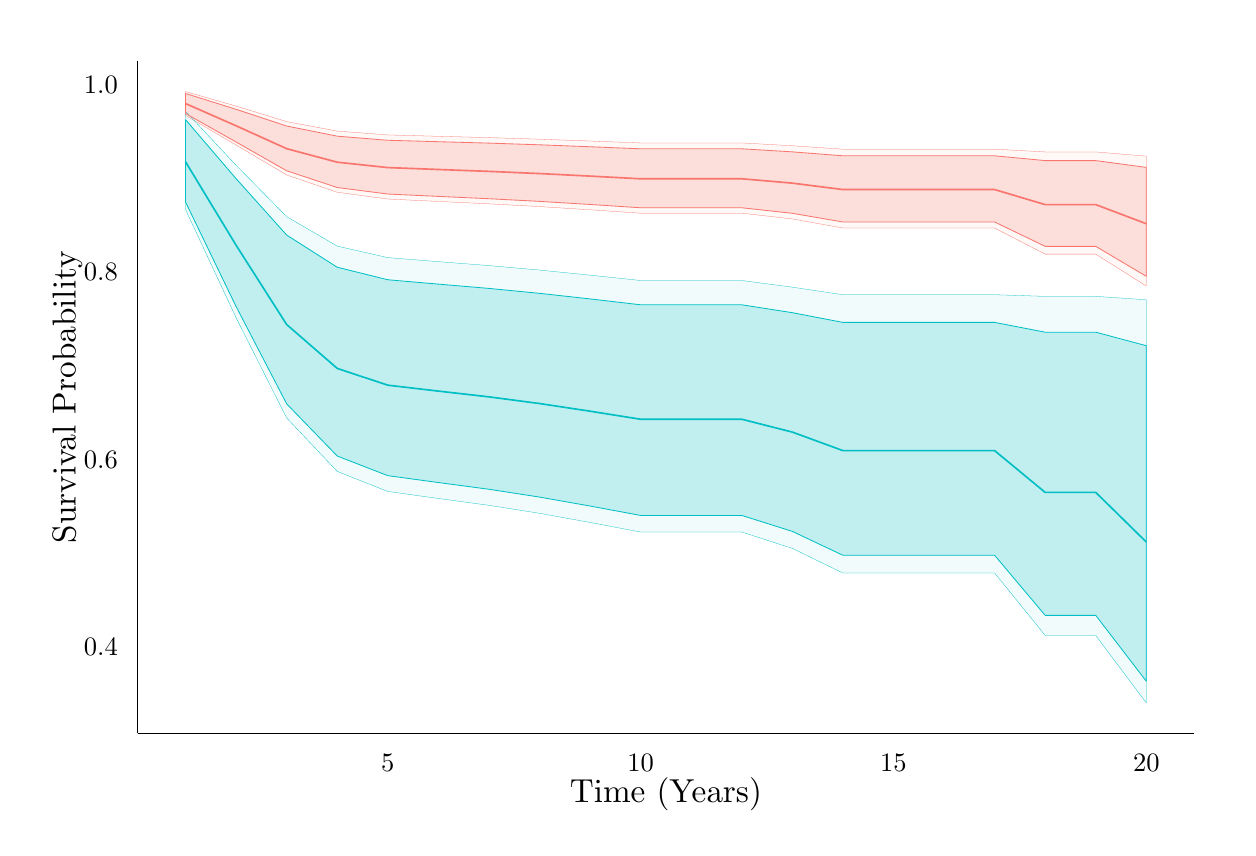
\begin{tikzpicture}[x=1pt,y=1pt]
\definecolor{fillColor}{RGB}{255,255,255}
\path[use as bounding box,fill=fillColor,fill opacity=0.00] (0,0) rectangle (433.62,289.08);
\begin{scope}
\path[clip] (  0.00,  0.00) rectangle (433.62,289.08);
\definecolor{drawColor}{RGB}{255,255,255}
\definecolor{fillColor}{RGB}{255,255,255}

\path[draw=drawColor,line width= 0.6pt,line join=round,line cap=round,fill=fillColor] (  0.00,  0.00) rectangle (433.62,289.08);
\end{scope}
\begin{scope}
\path[clip] ( 39.69, 34.03) rectangle (421.57,277.03);
\definecolor{fillColor}{RGB}{255,255,255}

\path[fill=fillColor] ( 39.69, 34.03) rectangle (421.58,277.03);
\definecolor{drawColor}{RGB}{248,118,109}

\path[draw=drawColor,line width= 0.6pt,line join=round] ( 57.05,261.65) --
	( 75.32,253.62) --
	( 93.59,245.35) --
	(111.86,240.46) --
	(130.13,238.52) --
	(148.41,237.83) --
	(166.68,237.15) --
	(184.95,236.36) --
	(203.22,235.44) --
	(221.49,234.47) --
	(239.77,234.47) --
	(258.04,234.47) --
	(276.31,232.90) --
	(294.58,230.58) --
	(312.86,230.58) --
	(331.13,230.58) --
	(349.40,230.58) --
	(367.67,225.14) --
	(385.94,225.14) --
	(404.22,218.23);
\definecolor{drawColor}{RGB}{0,191,196}

\path[draw=drawColor,line width= 0.6pt,line join=round] ( 57.05,240.59) --
	( 75.32,210.45) --
	( 93.59,181.80) --
	(111.86,165.95) --
	(130.13,159.89) --
	(148.41,157.75) --
	(166.68,155.67) --
	(184.95,153.26) --
	(203.22,150.49) --
	(221.49,147.58) --
	(239.77,147.58) --
	(258.04,147.58) --
	(276.31,142.94) --
	(294.58,136.25) --
	(312.86,136.25) --
	(331.13,136.25) --
	(349.40,136.25) --
	(367.67,121.15) --
	(385.94,121.15) --
	(404.22,103.21);
\definecolor{drawColor}{RGB}{248,118,109}
\definecolor{fillColor}{RGB}{248,118,109}

\path[draw=drawColor,line width= 0.1pt,line join=round,line cap=round,fill=fillColor,fill opacity=0.05] ( 57.05,265.99) --
	( 75.32,260.74) --
	( 93.59,255.13) --
	(111.86,251.71) --
	(130.13,250.32) --
	(148.41,249.83) --
	(166.68,249.35) --
	(184.95,248.78) --
	(203.22,248.12) --
	(221.49,247.43) --
	(239.77,247.43) --
	(258.04,247.43) --
	(276.31,246.41) --
	(294.58,245.17) --
	(312.86,245.17) --
	(331.13,245.17) --
	(349.40,245.17) --
	(367.67,244.18) --
	(385.94,244.18) --
	(404.22,242.65) --
	(404.22,195.72) --
	(385.94,207.25) --
	(367.67,207.25) --
	(349.40,216.67) --
	(331.13,216.67) --
	(312.86,216.67) --
	(294.58,216.67) --
	(276.31,219.96) --
	(258.04,222.04) --
	(239.77,222.04) --
	(221.49,222.04) --
	(203.22,223.27) --
	(184.95,224.43) --
	(166.68,225.42) --
	(148.41,226.28) --
	(130.13,227.16) --
	(111.86,229.60) --
	( 93.59,235.86) --
	( 75.32,246.65) --
	( 57.05,257.37) --
	cycle;
\definecolor{drawColor}{RGB}{0,191,196}
\definecolor{fillColor}{RGB}{0,191,196}

\path[draw=drawColor,line width= 0.1pt,line join=round,line cap=round,fill=fillColor,fill opacity=0.05] ( 57.05,258.85) --
	( 75.32,239.34) --
	( 93.59,220.79) --
	(111.86,210.14) --
	(130.13,205.99) --
	(148.41,204.53) --
	(166.68,203.11) --
	(184.95,201.49) --
	(203.22,199.65) --
	(221.49,197.72) --
	(239.77,197.72) --
	(258.04,197.72) --
	(276.31,195.31) --
	(294.58,192.58) --
	(312.86,192.58) --
	(331.13,192.58) --
	(349.40,192.58) --
	(367.67,191.99) --
	(385.94,191.99) --
	(404.22,190.75) --
	(404.22, 45.08) --
	(385.94, 69.47) --
	(367.67, 69.47) --
	(349.40, 92.02) --
	(331.13, 92.02) --
	(312.86, 92.02) --
	(294.58, 92.02) --
	(276.31,100.91) --
	(258.04,106.83) --
	(239.77,106.83) --
	(221.49,106.83) --
	(203.22,110.29) --
	(184.95,113.60) --
	(166.68,116.48) --
	(148.41,118.95) --
	(130.13,121.49) --
	(111.86,128.73) --
	( 93.59,148.04) --
	( 75.32,184.25) --
	( 57.05,223.34) --
	cycle;
\definecolor{drawColor}{RGB}{248,118,109}
\definecolor{fillColor}{RGB}{248,118,109}

\path[draw=drawColor,line width= 0.3pt,line join=round,line cap=round,fill=fillColor,fill opacity=0.20] ( 57.05,265.29) --
	( 75.32,259.58) --
	( 93.59,253.54) --
	(111.86,249.87) --
	(130.13,248.39) --
	(148.41,247.87) --
	(166.68,247.36) --
	(184.95,246.75) --
	(203.22,246.05) --
	(221.49,245.31) --
	(239.77,245.31) --
	(258.04,245.31) --
	(276.31,244.20) --
	(294.58,242.78) --
	(312.86,242.78) --
	(331.13,242.78) --
	(349.40,242.78) --
	(367.67,241.04) --
	(385.94,241.04) --
	(404.22,238.59) --
	(404.22,199.22) --
	(385.94,210.06) --
	(367.67,210.06) --
	(349.40,218.86) --
	(331.13,218.86) --
	(312.86,218.86) --
	(294.58,218.86) --
	(276.31,222.00) --
	(258.04,224.00) --
	(239.77,224.00) --
	(221.49,224.00) --
	(203.22,225.19) --
	(184.95,226.31) --
	(166.68,227.27) --
	(148.41,228.11) --
	(130.13,228.96) --
	(111.86,231.32) --
	( 93.59,237.36) --
	( 75.32,247.76) --
	( 57.05,258.06) --
	cycle;
\definecolor{drawColor}{RGB}{0,191,196}
\definecolor{fillColor}{RGB}{0,191,196}

\path[draw=drawColor,line width= 0.3pt,line join=round,line cap=round,fill=fillColor,fill opacity=0.20] ( 57.05,255.84) --
	( 75.32,234.50) --
	( 93.59,214.14) --
	(111.86,202.51) --
	(130.13,197.99) --
	(148.41,196.41) --
	(166.68,194.86) --
	(184.95,193.08) --
	(203.22,191.07) --
	(221.49,188.94) --
	(239.77,188.94) --
	(258.04,188.94) --
	(276.31,186.09) --
	(294.58,182.58) --
	(312.86,182.58) --
	(331.13,182.58) --
	(349.40,182.58) --
	(367.67,179.04) --
	(385.94,179.04) --
	(404.22,174.15) --
	(404.22, 52.90) --
	(385.94, 76.72) --
	(367.67, 76.72) --
	(349.40, 98.43) --
	(331.13, 98.43) --
	(312.86, 98.43) --
	(294.58, 98.43) --
	(276.31,107.06) --
	(258.04,112.83) --
	(239.77,112.83) --
	(221.49,112.83) --
	(203.22,116.22) --
	(184.95,119.46) --
	(166.68,122.28) --
	(148.41,124.71) --
	(130.13,127.20) --
	(111.86,134.29) --
	( 93.59,153.15) --
	( 75.32,188.29) --
	( 57.05,226.05) --
	cycle;
\end{scope}
\begin{scope}
\path[clip] (  0.00,  0.00) rectangle (433.62,289.08);
\definecolor{drawColor}{RGB}{0,0,0}

\path[draw=drawColor,line width= 0.6pt,line join=round] ( 39.69, 34.03) --
	( 39.69,277.03);
\end{scope}
\begin{scope}
\path[clip] (  0.00,  0.00) rectangle (433.62,289.08);
\definecolor{drawColor}{RGB}{0,0,0}

\node[text=drawColor,anchor=base east,inner sep=0pt, outer sep=0pt, scale=  0.96] at ( 32.57, 62.24) {0.4};

\node[text=drawColor,anchor=base east,inner sep=0pt, outer sep=0pt, scale=  0.96] at ( 32.57,129.92) {0.6};

\node[text=drawColor,anchor=base east,inner sep=0pt, outer sep=0pt, scale=  0.96] at ( 32.57,197.61) {0.8};

\node[text=drawColor,anchor=base east,inner sep=0pt, outer sep=0pt, scale=  0.96] at ( 32.57,265.30) {1.0};
\end{scope}
\begin{scope}
\path[clip] (  0.00,  0.00) rectangle (433.62,289.08);
\definecolor{drawColor}{RGB}{0,0,0}

\path[draw=drawColor,line width= 0.6pt,line join=round] ( 39.69, 34.03) --
	(421.57, 34.03);
\end{scope}
\begin{scope}
\path[clip] (  0.00,  0.00) rectangle (433.62,289.08);
\definecolor{drawColor}{RGB}{0,0,0}

\node[text=drawColor,anchor=base,inner sep=0pt, outer sep=0pt, scale=  0.96] at (130.13, 20.31) {5};

\node[text=drawColor,anchor=base,inner sep=0pt, outer sep=0pt, scale=  0.96] at (221.49, 20.31) {10};

\node[text=drawColor,anchor=base,inner sep=0pt, outer sep=0pt, scale=  0.96] at (312.86, 20.31) {15};

\node[text=drawColor,anchor=base,inner sep=0pt, outer sep=0pt, scale=  0.96] at (404.22, 20.31) {20};
\end{scope}
\begin{scope}
\path[clip] (  0.00,  0.00) rectangle (433.62,289.08);
\definecolor{drawColor}{RGB}{0,0,0}

\node[text=drawColor,anchor=base,inner sep=0pt, outer sep=0pt, scale=  1.20] at (230.63,  9.03) {Time (Years)};
\end{scope}
\begin{scope}
\path[clip] (  0.00,  0.00) rectangle (433.62,289.08);
\definecolor{drawColor}{RGB}{0,0,0}

\node[text=drawColor,rotate= 90.00,anchor=base,inner sep=0pt, outer sep=0pt, scale=  1.20] at ( 17.30,155.53) {Survival Probability};
\end{scope}
\end{tikzpicture}
